\index{Preferences!Test Case Diagram}
\index{Test Case Diagram!Preferences}

In the \gdcase{} diagram preferences page (\bxfigref{diagramprefs}), you can configure:

\begin{figure}[h]
\begin{center}
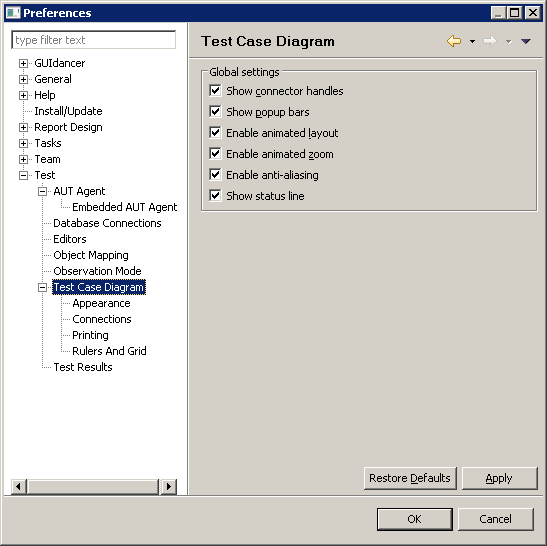
\includegraphics[width=12.5cm]{Tasks/Preferences/PS/diagramprefs}
\caption{Diagram Preference Dialog}
\label{diagramprefs}
\end{center}
\end{figure}

\begin{description}
\item [Connector handles:]{When this option is checked, you will see the connection arrows to add notes when an element is selected in your model. Click on a connector and drag to create a new note.}
\item [Pop up bars:]{When this option is checked, you will see a pop-up with the options to add parameters and \gdcase{} referenced when an element is selected in your model. Clicking on the \bxname{add parameter} or the \bxname{add \gdcase{} reference} icon will add the element you choose to the currently selected item. }
\item [Animated layout:]{When this option is activated, the arrangement of the items in the diagram will be animated when you click the \bxcaption{Arrange} button in the toolbar. }
\item [Animated zoom:]{When this option is activated, zooming into or out of the diagram will be animated. }
\item [Anti-aliasing:]{Use this option with higher-performance machines to smooth the lines connecting elements in the model. Machines with lower performance should deactivate this option. }
\end{description}

\subsubsection{\gdcase{} diagram appearance preferences}
\gdhelpid{prefPageTCDAppearanceContextId}{Test Case Diagram Appearance Preferences}
On the appearance preference page for the \gdcase{} diagram, you can specify which colors should be used within the model, for text and lines in the notes and in general. 

\begin{figure}[h]
\begin{center}
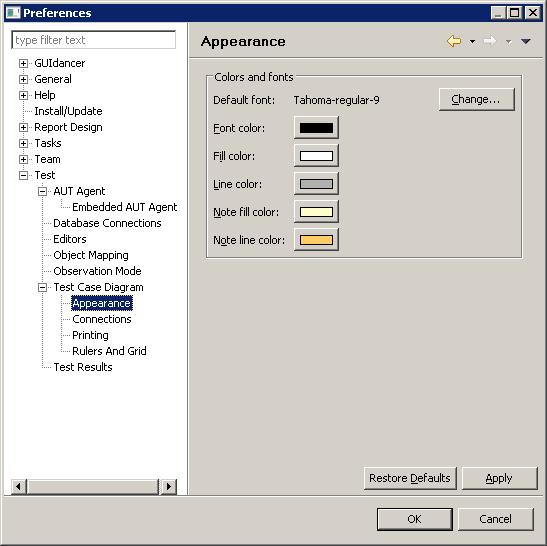
\includegraphics[width=12.5cm]{Tasks/Preferences/PS/diagramappearanceprefs}
\caption{Diagram Appearance Preference Dialog}
\label{diagramappearanceprefs}
\end{center}
\end{figure}

\subsubsection{\gdcase{} diagram connections preferences}
\gdhelpid{prefPageTCDConnectionsContextId}{Test Case Diagram Connections Preferences}
Use this preference page to specify how you would like the connections to appear in your model. 
\begin{description}
\item [Oblique]{displays the connectors as direct, straight lines between the connected elements. }
\item [Rectilinear]{displays connecting lines at right angles between the connected elements.}
\end{description}


\subsubsection{\gdcase{} diagram printing preferences}
\gdhelpid{prefPageTCDPrintingContextId}{Test Case Diagram Printing Preferences}
If you are planning on printing your \gdcase{} model, you can configure the print preferences in this page. For example, you can set the page orientation to portrait or landscape and use the context-sensitive menu in the model to view the page boundaries for your chosen orientation. 

\begin{figure}[h]
\begin{center}
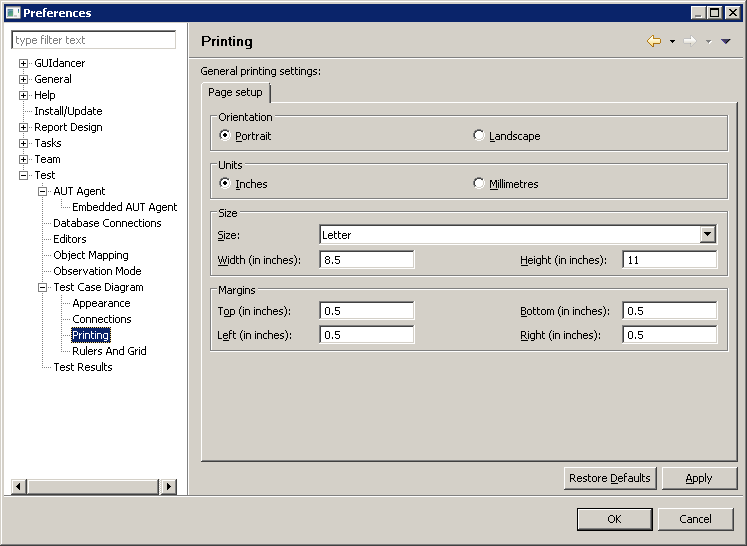
\includegraphics[width=12.5cm]{Tasks/Preferences/PS/diagramprintingprefs}
\caption{Diagram Printing Preference Dialog}
\label{diagramprintingprefs}
\end{center}
\end{figure}

\subsubsection{\gdcase{} diagram rulers and grid preferences}
\gdhelpid{prefPageTCDRulersContextId}{Test Case Diagram Rulers and Grid Preferences}
In this preference page, you can specify whether you want to see the rulers and the grid for new diagrams. In the ruler settings, you can also specify the ruler units as centimeters, inches or pixels. 

Within the grid options, you can choose whether elements should snap to the grid (\bxname{snap to grid}), or to each other (\bxname{snap to shape}). The snap to shape option displays a horizontal or vertical line when an element is moved close to another element. The line can be used to line elements up with each other. 

The grid spacing can also be altered to decrease or increase the size of the grid blocks.  

\begin{figure}[h]
\begin{center}
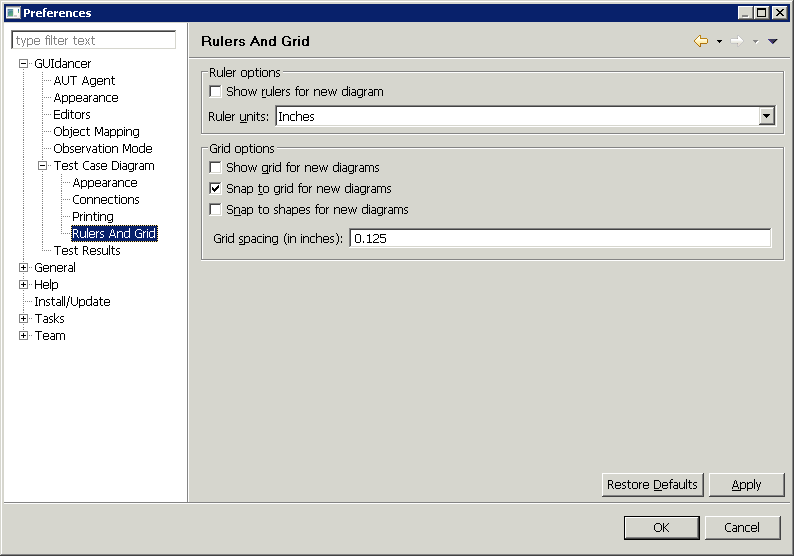
\includegraphics[width=12.5cm]{Tasks/Preferences/PS/diagramrulersprefs}
\caption{Diagram Rulers and Grids Preference Dialog}
\label{diagramrulersprefs}
\end{center}
\end{figure}
